% This is samplepaper.tex, a sample chapter demonstrating the
% LLNCS macro package for Springer Computer Science proceedings;
% Version 2.20 of 2017/10/04
%
\documentclass[runningheads]{llncs}
%
\usepackage{graphicx}
\usepackage{amsmath}
\usepackage{amsfonts}
\usepackage{float}
% Used for displaying a sample figure. If possible, figure files should
% be included in EPS format.
%
% If you use the hyperref package, please uncomment the following line
% to display URLs in blue roman font according to Springer's eBook style:
% \renewcommand\UrlFont{\color{blue}\rmfamily}

\begin{document}
%
\title{DKT8x8: A Dataset for Digital Watermarking Using Krawtchouk Moments}
%
%\titlerunning{Abbreviated paper title}
% If the paper title is too long for the running head, you can set
% an abbreviated paper title here
%
\author{Ernesto Avila-Domenech\inst{1}\orcidID{0000-0002-4797-289X} \and
Alberto Taboada-Crispi\inst{2}\orcidID{0000-0002-7797-1441} \and
Anier Soria-Lorente\inst{1}\orcidID{0000-0003-3488-3094}}
%
\authorrunning{E. Avila-Domenech et al.}
% First names are abbreviated in the running head.
% If there are more than two authors, 'et al.' is used.
%
\institute{Universidad de Granma, Carretera Central v{\'i}a Holgu{\'i}n Km $\frac{1}{2}$, Granma, Cuba \email{\{eadomenech, asorial1983\}@gmail.com}\\ \and
Universidad Central de Las Villas, Villa Clara, Cuba\\
\email{\{ataboada\}@uclv.edu.cu}}
%
\maketitle              % typeset the header of the contribution
%
\begin{abstract}
In this paper we present a new image block dataset DKT8x8. DKT8x8 containing over 90000 $8\times 8$ color images from 9 class. The dataset was obtained by dividing into $8\times 8$ blocks each of the images corresponding to the DIBCO 2017 dataset and calculating the coefficient and embedding strength values so that the balance between PSNR and BER. We first describe the dataset, its collection and construction. Secondly, we provide key descriptive statistics. Finally, we evaluate the dataset on digital watermarking method and present related experimental results.

\keywords{Dataset  \and Digital watermarking \and Image.}
\end{abstract}
%
%
%
\section{Introduction}
The rest of the paper is organised as follow; Section 2 describes the proposed method including fragil watermarking and robust watermarking. Experimental results are given in Section 3 and Section 4 concludes the paper.

Kaggle provides a huge number of competitions on different data science problems \cite{Subramanian2018}.

\section{Data characteristics}

Based of works \cite{avila2018watermarking}, to classify the $8\times 8$ blocks according to the optimal marking parameters is proposed in this paper. For capturing spatial information of $8\times 8$ blocks.

\subsection*{Krawtchouk moments}
The Krawtchouk moments were introduced by Yap in \cite{Yap2003}. These orthogonal moments satisfy the following recurrence relation
\begin{multline*}
\alpha_n(Np-2np+n-x)\overline{K}_{n}^{p,N}(x) \\= p(n-N)\overline{K}_{n+1}^{p,N}(x)+\beta_n n(1-p)\overline{K}_{n-1}^{p,N}(x),\quad n\geq 1,
\end{multline*}
with initial conditions 
\begin{equation*}
\overline{K}_{0}^{p,N}(x) = \sqrt{w^{p,N}(x)p^{-1}},
\end{equation*}	
and
\begin{equation*}
\overline{K}_{1}^{p,N}(x) = (Np-x)(Np)^{-1}\sqrt{w^{p,N}(x)(1-p)(Np)^{-1}},
\end{equation*}
where $\alpha_n = \sqrt{\frac{(1-p)(n+1)}{p(N-n)}}$, $\beta_n = \sqrt{\frac{(1-p)^2(n+1)n}{p^2(N-n)_2}}$, $w^{p,N}(x) = \binom{N}{x}p^x(1-p)^{N-x}$ and $0<p<1$.

The Krawtchouk moment of order $(m+n)$ of an image $f(x,y)$ with $M\times N$ pixels is defined as

\begin{equation}
K_{mn}=\sum_{x=0}^{M-1}\sum_{y=0}^{N-1}f(x,y)\overline{K}_{m}^{p,M}(x)\overline{K}_{n}^{q,N}(y),
\label{DKT}
\end{equation}
where $m\in \left[ 0,M-1\right] $ and $n\in \left[ 0,N-1\right] $.

The image $f(x,y)$ can be reconstructed using
\begin{equation}
f(x,y)=\sum_{m=0}^{M-1}\sum_{n=0}^{N-1}K_{mn}\overline{K}_{m}^{p,M}(x)\overline{K}_{n}^{q,N}(y),
\label{IDKT}
\end{equation}
where $x\in \left[ 0,M-1\right] $ and $y\in \left[ 0,N-1\right] $.

The lower order Krawtchouk moments store information of a specific region-of-interest of an image, the higher order moments store information of the rest of the image. Therefore, by reconstructing the image from the lower order moments and discarding the higher order moments, a sub-image can be extracted from the subject image. For each additional moment used in reconstructing the image, the square error of the reconstructed image is reduced \cite{Yap2003}.

The set of lower order Krawtchouk moments is generally the set of perceptually significant components of the image. This choice ensures that the watermark is robust to attacks \cite{Yap2004}.

\subsection*{Dither modulation quantization}
Dither modulation quantization technique is one of the most popular in the watermarking. It has good performance on following requirements of watermarking: perceptibility ratio, data payload, robustness, and blind extraction. The combination of dither modulation quantization with different transformation domain watermarking methods also improves watermark extraction capability \cite{chen2001quantization}. 

One bit of the watermark can be embedded as
\begin{equation}
|C{}_{0}^{'}(k_{1},k_{2})|=\begin{cases}
2\Delta\times round(\frac{|C{}_{0}(k_{1},k_{2})|}{2\Delta})+\frac{\Delta}{2}, & if\:W(i,j)=1\\
2\Delta\times round(\frac{|C{}_{0}(k_{1},k_{2})|}{2\Delta})-\frac{\Delta}{2} & if\:W(i,j)=0
\end{cases},
\label{DMEm}
\end{equation}
where $\Delta$ is the quantization step controlling the embedding strength of the watermark bit, $|\cdot|$ is the absolute operator, $round(\cdot)$ denotes the rounding operation to the nearest integer, $W(i,j)$ is the watermark bit at the position $(i,j)$ and $C{}_{0}^{'}(k_{1},k_{2})$ is the modified block.

To extract the watermark it is used
\begin{equation}
W^{*}(i,j)=arg_{\sigma\in\{0,1\}}min(|C_{0}^{''}(k_{1},k_{2})|_{\sigma}-|C_{0}^{*}(k_{1},k_{2})|)
\label{DMEx},
\end{equation}
where $C_{0}^{*}(k_{1},k_{2})$ is the extracted watermark and $|C_{0}^{''}(k_{1},k_{2})|_{\sigma}$ is defined as
\begin{equation}
|C_{0}^{''}(k_{1},k_{2})|_{\sigma}=\begin{cases}
2\Delta\times round(\frac{|C_{0}^{*}(k_{1},k_{2})|}{2\Delta})+\frac{\Delta}{2}, & if\:\sigma=1\\
2\Delta\times round(\frac{|C_{0}^{*}(k_{1},k_{2})|}{2\Delta})-\frac{\Delta}{2} & if\:\sigma=0
\end{cases}.
\end{equation}

\subsection*{Watermark embedding scheme}
\begin{itemize}
	\item[\checkmark] The block of $8\times 8$ pixels is transformed from RGB to YCbCr color space, and the Y component, corresponding to the luminance information is seleted.
	\item[\checkmark] The Krawtchouk moments of selected blocks are determined by Eq.~\ref{DKT}.
	\item[\checkmark] Watermark bit is embedded in the selected block moments using Dither modulation (see Eq.~\ref{DMEm}).
	\item[\checkmark] Watermarked blocks can be obtained using Eq.~\ref{IDKT}.
	\item[\checkmark] The last step is to transform the YCbCr to RGB space to obtain RGB watermarked image.
\end{itemize}

\subsection*{Watermark extraction}
\begin{itemize}
	\item[\checkmark] The watermarked image is transformed from the RGB to the YCbCr color space and the Y component is divided into $8\times 8$ pixels blocks.
	\item[\checkmark] The Krawtchouk moments of selected blocks are determined.
	\item[\checkmark] Scrambled watermark bits are obtained with the selected block moments using Dither modulation (see Eq.~\ref{DMEx}).
	\item[\checkmark] Finally, QR code watermark is constructed with the scrambled bits using Arnold transform.
\end{itemize}

\section{Dataset creation}

A new dataset of $8\times 8$ color images of 100000 from 10 categories, with 10000 images per category was create. The training set has 90000 images and the valid set has 10000 images. The dataset was obtained by dividing into $8\times 8$ blocks each of the images corresponding to the DIBCO 2017 dataset and calculating the coef and delta values so that the balance between PSNR and BER represented as $FO$ were the highest possible values for each of the blocks.

\begin{equation}
FO = (PSNR/160 + \alpha + \beta)/3,
\label{FA}
\end{equation}
where $PSNR$ is the logarithmic value of ratio between signal and noise, $ \alpha $ is the success in extracting the watermark from the watermarked image without noise and $ \beta $ is the success in extracting the watermark from the watermarked image after applying a JPEG compression with QF= 25{\%}.

Como promedio existirian 1200 imagenes por clases.

Se propondrian como clases las siguientes:
\begin{enumerate}
	\item 16\_100 (5816)
	\item 19\_67 (5078)
	\item 19\_73 (4640)
	\item 19\_78 (5141)
	\item 19\_82 (5306)
	\item 19\_85 (4465)
	\item 19\_90 (5093)
	\item 19\_98 (5063)
	\item 19\_115 (5058)
\end{enumerate}

\section{Descriptive statistics}

\begin{figure} [H]
	\begin{center}
		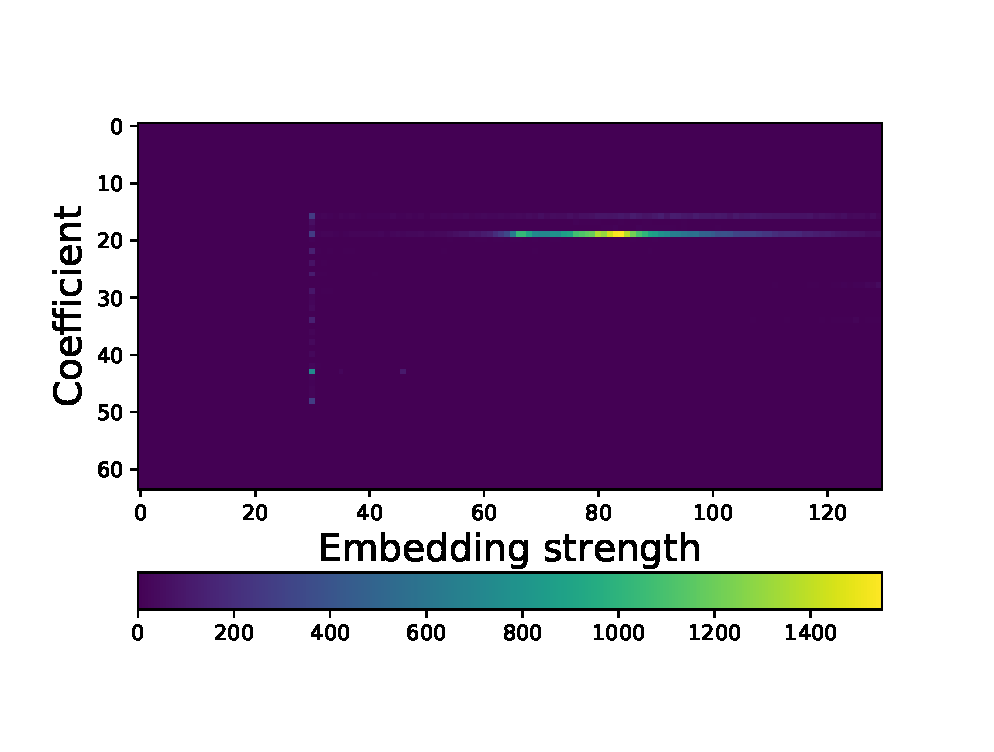
\includegraphics[width=\textwidth]{colormap.eps}
		\caption{Coefficient and embedding strength values.} \label{colormap}
	\end{center}
\end{figure}

\begin{figure} [H]
	\begin{center}
		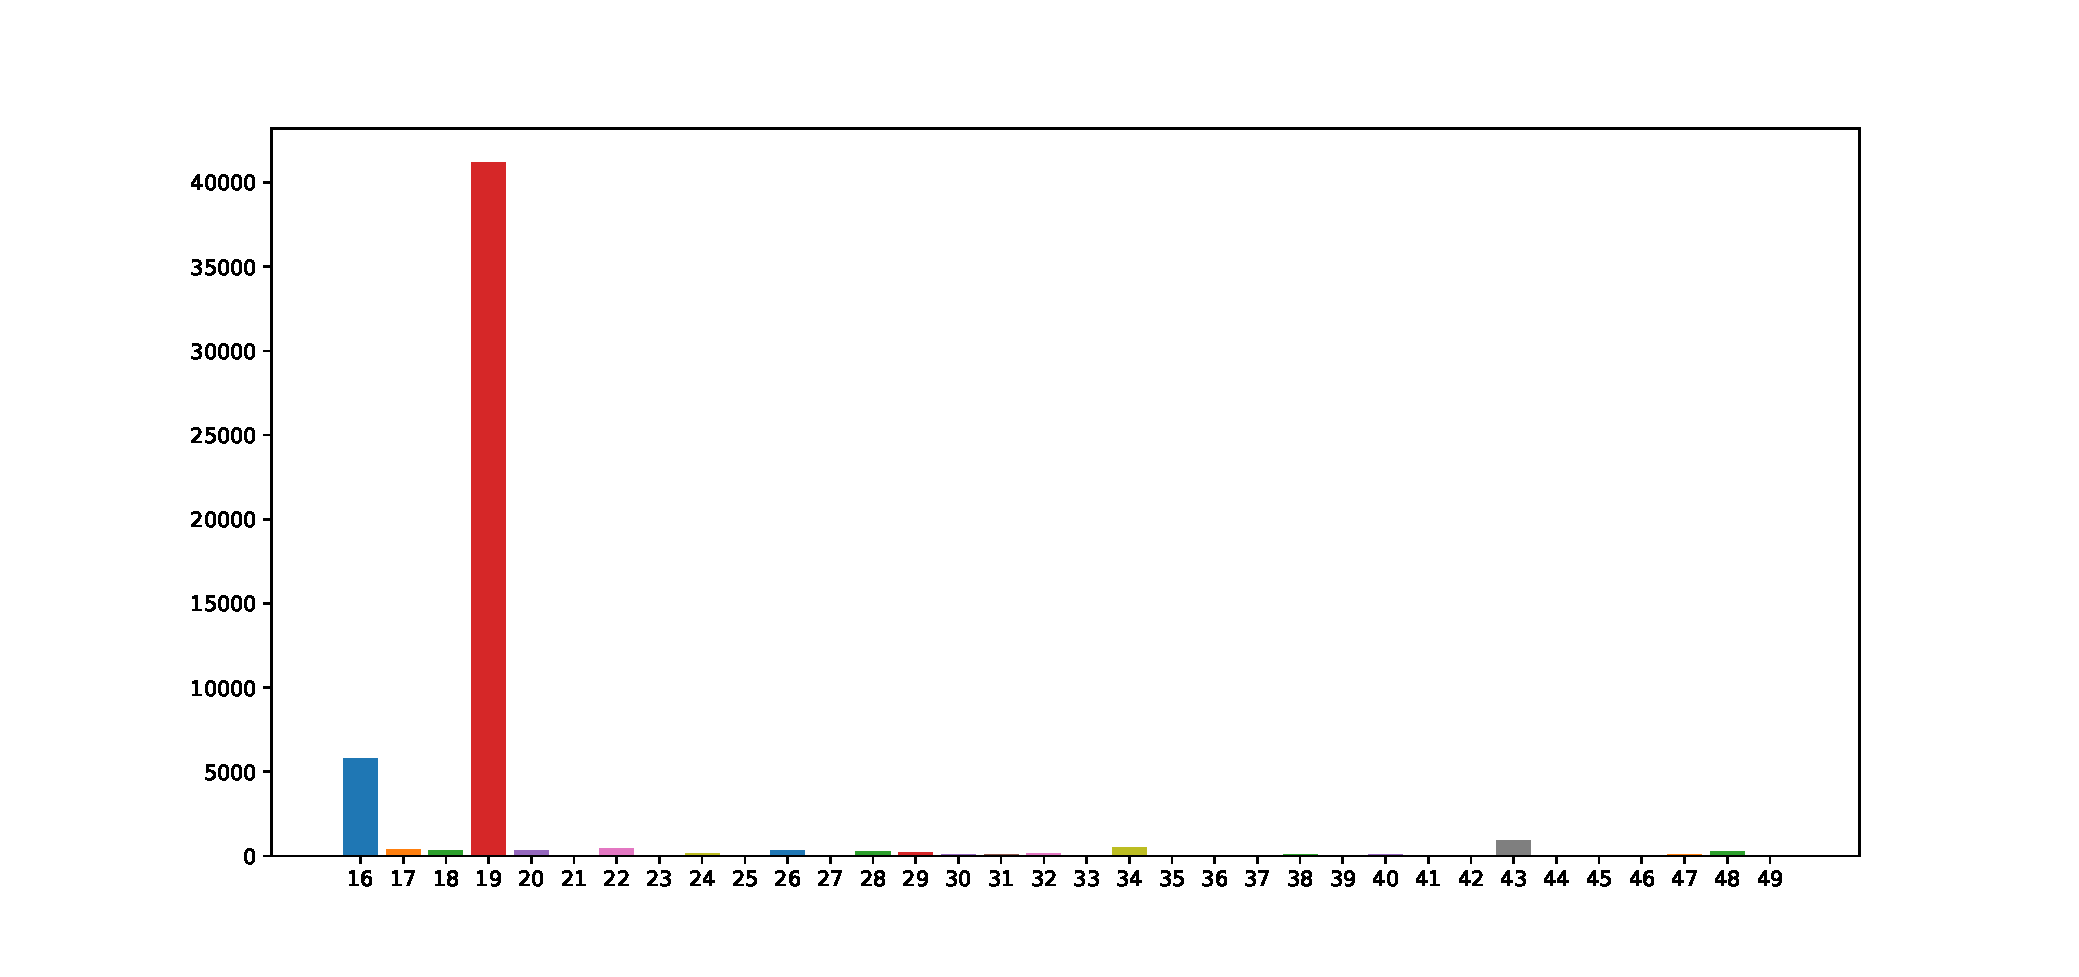
\includegraphics[width=\textwidth]{frequency_bar.eps}
		\caption{Coef and delta.} \label{frequency_bar}
	\end{center}
\end{figure}

\section{Experiments}

\begin{figure} [H]
	\begin{center}
		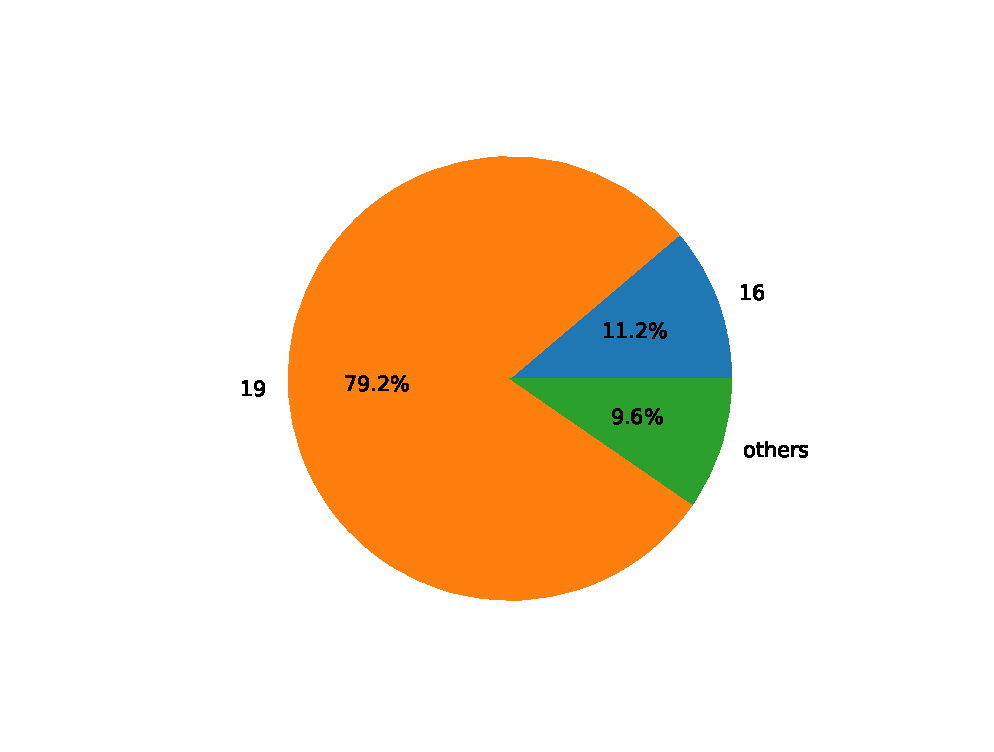
\includegraphics[width=0.7\textwidth]{pastel.eps}
		\caption{Coef and delta.} \label{pastel}
	\end{center}
\end{figure}

\section{Conclusions}
In this paper, a dual digital watermarking technique based on Neural Network and SHA-256 hash function was implemented. The results show a BER less than $0.005 \%$, so the extracted QR codes were decoded in $100\%$ of the $60$ analyzed images. In addition, the values corresponding to the PSNR were improved compared to previously presented papers.
%
% ---- Bibliography ----
%
% BibTeX users should specify bibliography style 'splncs04'.
% References will then be sorted and formatted in the correct style.
%
\bibliographystyle{splncs04}
\bibliography{mybibliography}
%
\end{document}
